\documentclass{beamer}
\usetheme{Madrid}

\usepackage{amsmath, amssymb, amsthm}
\usepackage{graphicx}
\usepackage{gensymb}
\usepackage[utf8]{inputenc}
\usepackage{hyperref}
\usepackage{tikz}
\usepackage{amsmath}

\title{6.4.12 Matgeo}
\author{AI25BTECH11012 - Garige Unnathi}
\date{}

\begin{document}

\frame{\titlepage}

% Question frame
\begin{frame}
\frametitle{Question}
Find the shortest distance between the lines
\begin{align*}
 \textbf{r} = \hat{i}+2\hat{j}+\hat{k} +\lambda(\hat{i}-\hat{j}+\hat{k})
\end{align*}
\begin{align*}
    \textbf{r} =  2\hat{i}-\hat{j}-\hat{k} +\mu(2\hat{i}-\hat{j}+2\hat{k})
\end{align*}

\end{frame}


% Solution steps
\begin{frame}
\frametitle{Solution}
\begin{align}
\textbf{$x_1$} = \begin{bmatrix}1 \\2 \\1\end{bmatrix} + \lambda\begin{bmatrix}1 \\-1 \\1\end{bmatrix}\\
\textbf{$x_2$} = \begin{bmatrix}2 \\-1 \\-1\end{bmatrix} + \mu\begin{bmatrix}2 \\ -1\\ 2\end{bmatrix}\\
\textbf{M} = \begin{bmatrix}1 & 2 \\ -1 & -1\\1 & 2\end{bmatrix} \\
\textbf{B}-\textbf{A} = \begin{bmatrix}1 \\ -3 \\-2\end{bmatrix}
\end{align}
\end{frame}

\begin{frame}
\frametitle{Solution}
\begin{align}
   \begin{bmatrix}\textbf{M} & \textbf{B-A}\end{bmatrix} = \begin{bmatrix}1 & 2 & 1 \\ -1 & -1 & -3\\1 & 2 & -2\end{bmatrix}\\
 R_3 = R_3 + R_2 \quad and \quad  R_2 = R_2 + R_1\\
 = \begin{bmatrix}1 & 2 & 1 \\ 0 & 1 & -3\\0 & 1 & -5\end{bmatrix}\\
    R_3 = R_3  - R_2 \\
 = \begin{bmatrix}1 & 2 & 1 \\ 0 & 1 & -3\\0 & 0 & -2\end{bmatrix}
\end{align}
\end{frame}

\begin{frame}
\frametitle{Solution}
as the rank of above matrix is 3 the lines are skew lines
\begin{align}
     \begin{bmatrix}1 & -1 & 1 \\ 2 & -1 & 2\end{bmatrix} \begin{bmatrix}1 & 2 \\ -1 & -1\\1 & 2\end{bmatrix}\kappa =  \begin{bmatrix}1 & -1 & 1 \\ 2 & -1 & 2\end{bmatrix} \begin{bmatrix}1 \\ -3 \\-2\end{bmatrix} \\
  \begin{bmatrix}3 & 5\\5 & 9\end{bmatrix}\kappa =  \begin{bmatrix}2 \\ 1\end{bmatrix}
\end{align}

The argumented matrix of the above matrix is 
\begin{align}
=  \begin{bmatrix}3 & 5 & 2\\5 & 9 & 1\end{bmatrix} \\
 R_2 = R_2 - \frac{5}{3}R_1 \quad and \quad R_1 = R_1 - \frac{15}{2}R_2\\
= \begin{bmatrix}3 & 0 & \frac{39}{2}\\0 & \frac{2}{3} & -\frac{7}{3}\end{bmatrix}
 \end{align}
 \end{frame}

 \begin{frame}
\frametitle{Solution}
 yeilding 
\begin{align}
    \begin{bmatrix}\lambda \\ -\mu\end{bmatrix} = \begin{bmatrix}\frac{13}{2} \\ -\frac{7}{2}\end{bmatrix}
\end{align}
\begin{align}
    \textbf{$x_1$} =\frac{1}{2} \begin{bmatrix}15 \\ -9 \\ 15\end{bmatrix} ,
        \textbf{$x_2$} =\frac{1}{2} \begin{bmatrix}18 \\ -9 \\ 12\end{bmatrix}
\end{align}
\end{frame}

 \begin{frame}
\frametitle{Solution}
The minimum distance between the lines is given by
\begin{align}
    \lVert \textbf{$x_2$} - \textbf{$x_1$} \rVert = \lVert \frac{1}{2}\begin{bmatrix}3 \\ 0 \\ -3\end{bmatrix}
     = \frac{3\sqrt{2}}{2}
\end{align}
\end{frame}

% Graphical representation
\begin{frame}

\frametitle{Graphical Representation}
\begin{center}
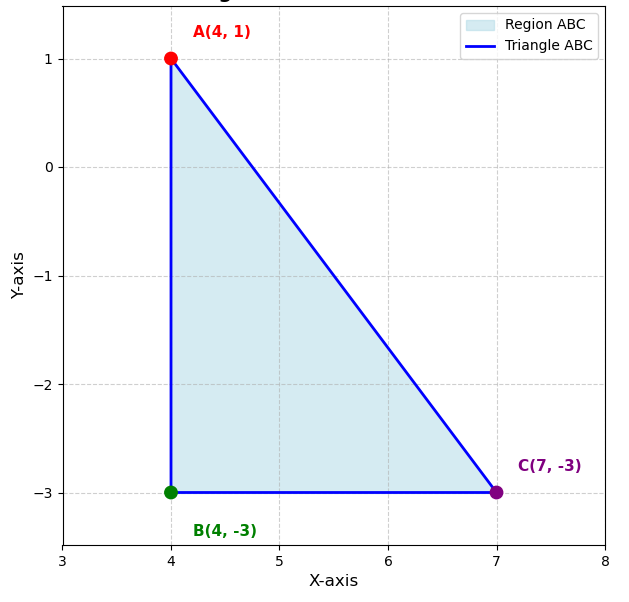
\includegraphics[width=0.6\linewidth]{/Users/unnathi/Documents/ee1030-2025/ai25btech11012/matgeo/6.4.12/figs/fig.png}
\end{center}
\end{frame}

\end{document}
